\subsection{Shallow Parabola-shaped Branches $f_\A$ and $f_\C$}
\label{sec:setup.quad.hyper.2}

\hl{
	To close the gaps in between the parameter regions in the sequences, the parameters of the function $g_L$ that governs the shape of the branches $f_\A$ and $f_\C$ is adjusted.
	The new fixed parameter values are $a_L = 4$ and $b_L = -\frac{1}{2}$.
	And the other fixed parameters stay the same as in the previous section.
}

\hl{One can see in} \Cref{fig:setup.quad.hyper.1.cobwebs} \hl{that the shape of the branches $f_\A$ and $f_\C$ is very steep}.
\hl{
	This is different from the branches $F_\A$ and $F_\C$ in the original model that were more shallow.
	The new fixed parameter values of $a_L$ and $b_L$ also cause the shape of the branches $f_\A$ and $f_\C$ to be more shallow.
}
\hl{One can see this in the cobweb diagrams in} \Cref{fig:setup.quad.hyper.2.cobwebs}.
\hl{
	The varied parameters are the same as in the previous section and therefore the parameter effects of $E_0$ and $\chi_0$ on the original model function are emulated well.
}
\hl{This was thoroughly described in the previous section,} \Cref{sec:setup.quad.hyper.1}.

\Cref{fig:setup.quad.hyper.2.period} \hl{shows 2D scans of periods associated with parameter regions in this model}.
\hl{
	It shows 2 different versions of scans in the same parameter range, $\alpha \in [0.275, 0.35]$ and $\beta \in [0.15, 0.1875]$.
}
\hl{The first scan in} \Cref{fig:setup.quad.hyper.2.period.full} \hl{shows the periods of the model as we have seen it also in the previous sections}.
\hl{The second scan in} \Cref{fig:setup.quad.hyper.2.period.halved} \hl{shows the periods of the same model but halved}.
\hl{This reveals ``type B'' parameter regions as they are associated with higher periods than the ``type A'' parameter regions of the same chains in the halved model}.
\hl{The reason for this is covered in-depth in} \Cref{sec:add.add.halved}, \hl{but for now only the fact that it reveals ``type B'' parameter regions is important}.

We can see in \Cref{fig:setup.quad.hyper.2.period.full}, that the gap between the ``type A'' parameter regions of a sequence \hl{of parameter regions associated} with the same period closed.
Also, there \hl{are sections of the chains where they} get narrower, \hl{for example at point $C$}.
\hl{
	In the original model one can observe the same narrowing of the chains.
	These narrower sections are ``type B'' parameter regions in the original model.
}


\Cref{fig:setup.quad.hyper.2.period.halved} \hl{reveals ``type B'' parameter regions in the quadratic model with compound parameters}.
\hl{
	We can see that ``type A'' and ``type B'' parameter regions alternate in the chains of parameter regions associated with the same period.
	Also, the ``type B'' parameter regions are at the narrower sections of the chains.
	This is exactly the same behavior one can observe in the original model when examining the types of the parameter regions making up the chains and their arrangement.
}

\hl{The period the chains are associated with also still increments in neighboring chains as was observed in the last section,} \Cref{sec:setup.quad.hyper.1}.
\hl{
	Therefore, this structure is similar to the \gls{pi} structure one can observe in the original model when looking at the periods associated with parameter regions and their types.
	But this is not the only characteristic of cycles.
	Therefore, the symbolic sequences of the cycles associated with the parameter regions making up the chains are analyzed next.
}

\begin{figure}
	\centering
	\subfloat[Model]{
		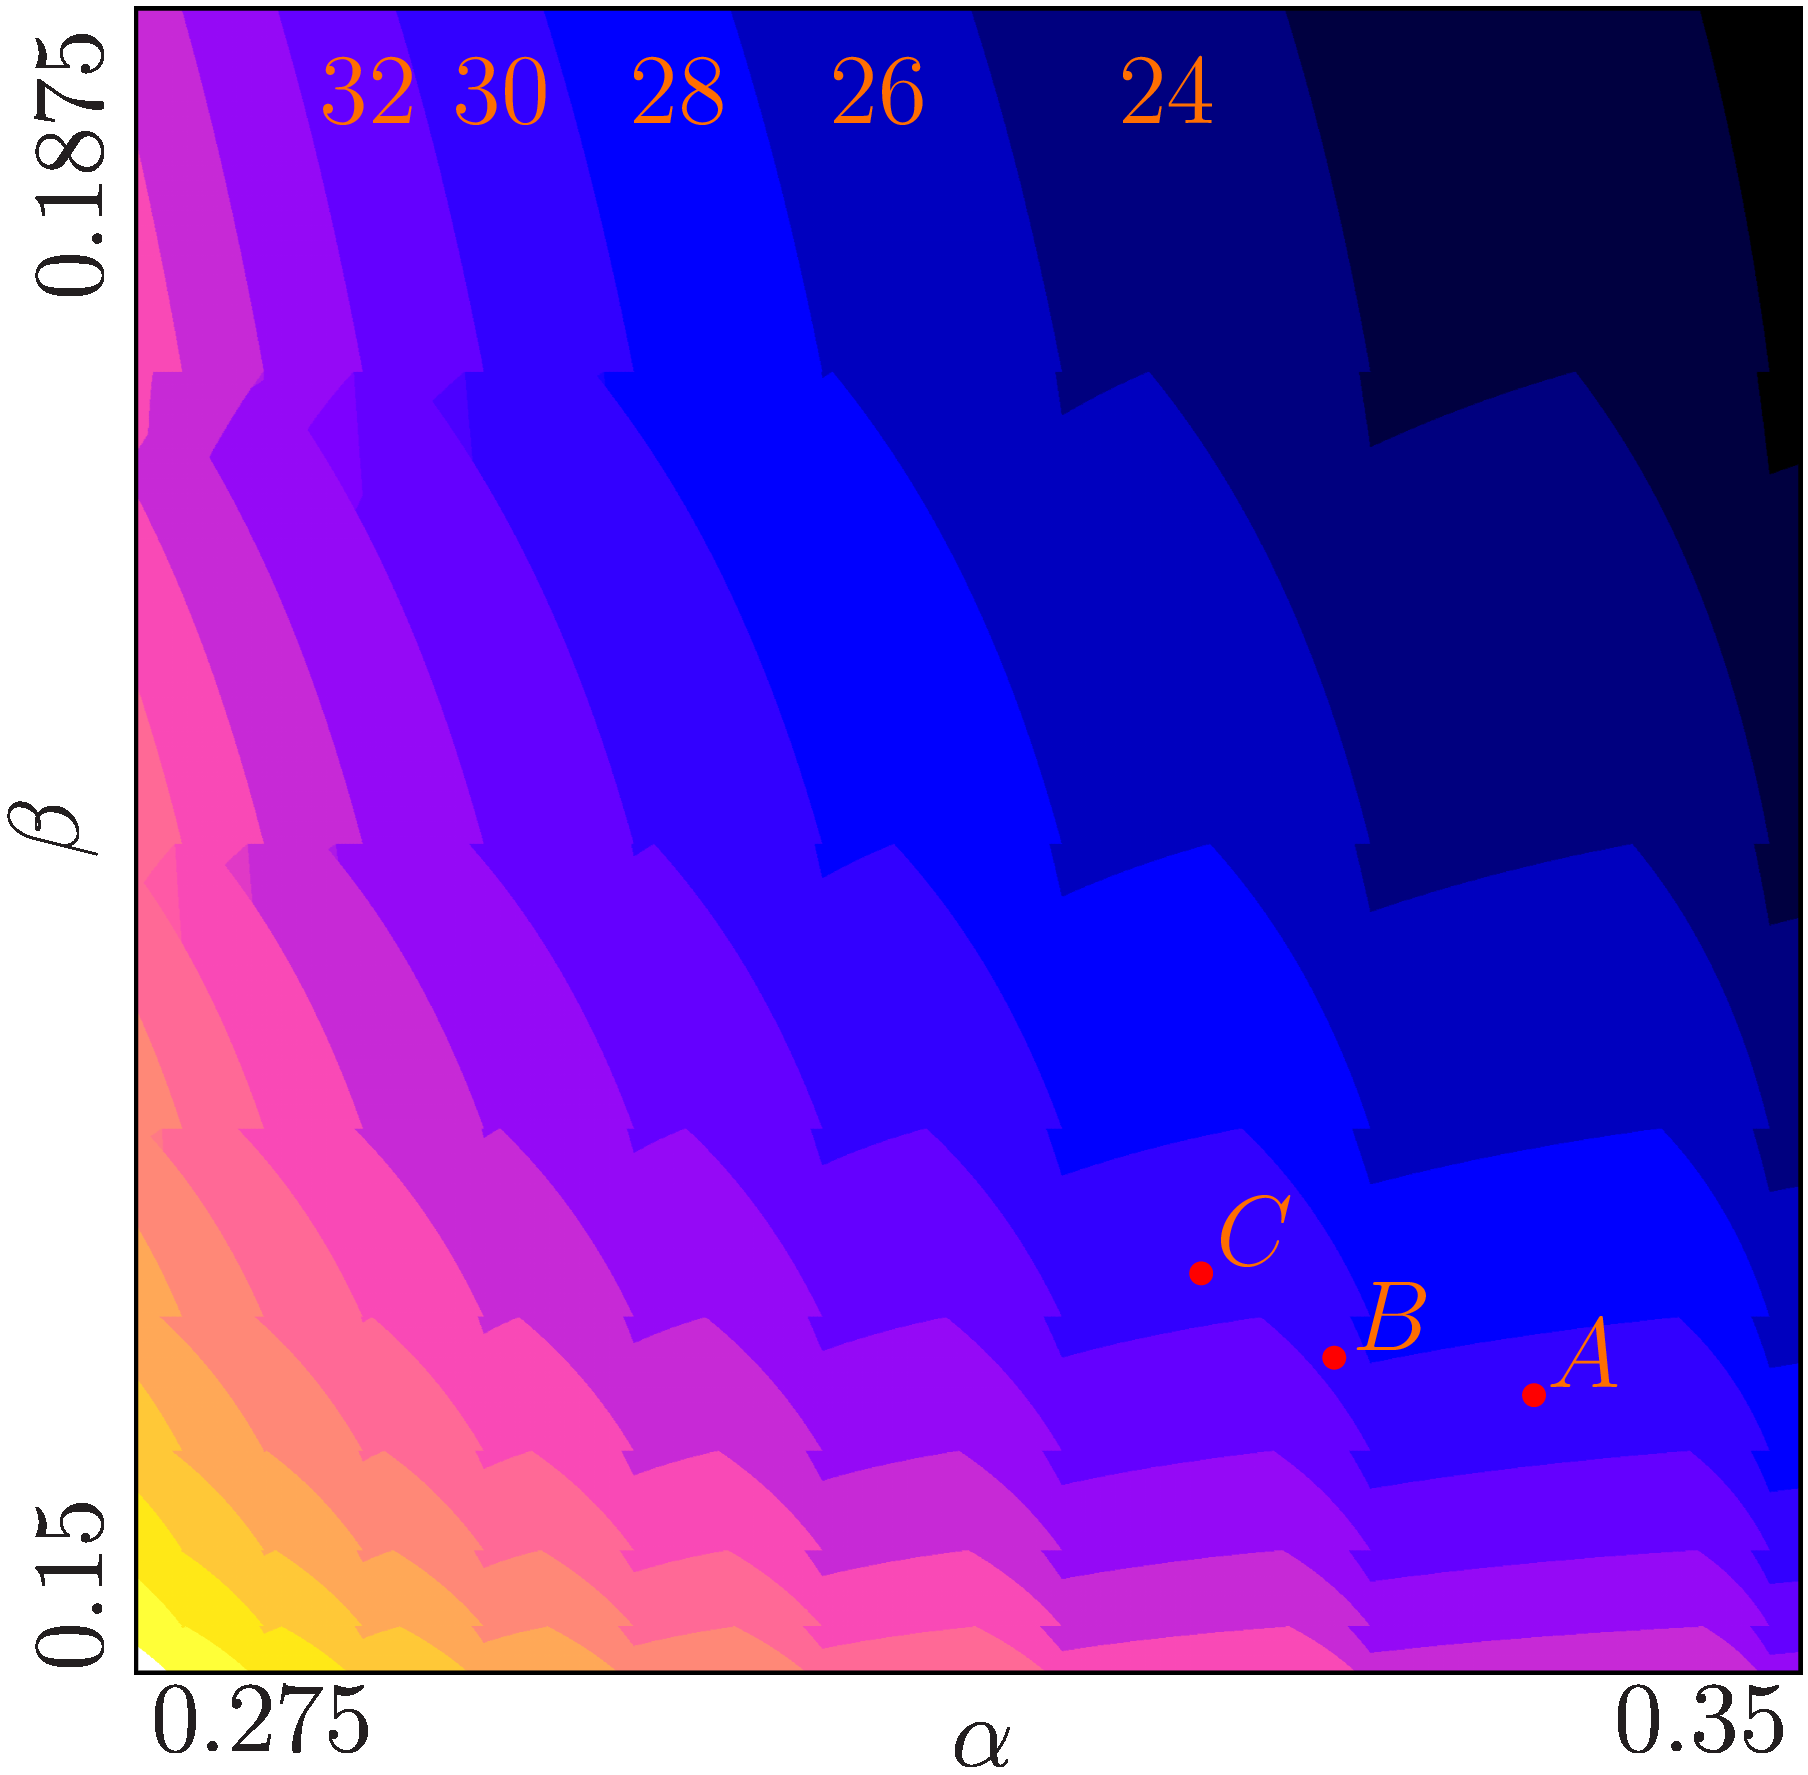
\includegraphics[width=.48 \textwidth]{../Figures/5/5.11a/result.png}
		\label{fig:setup.quad.hyper.2.period.full}
	}
	\subfloat[Halved model]{
		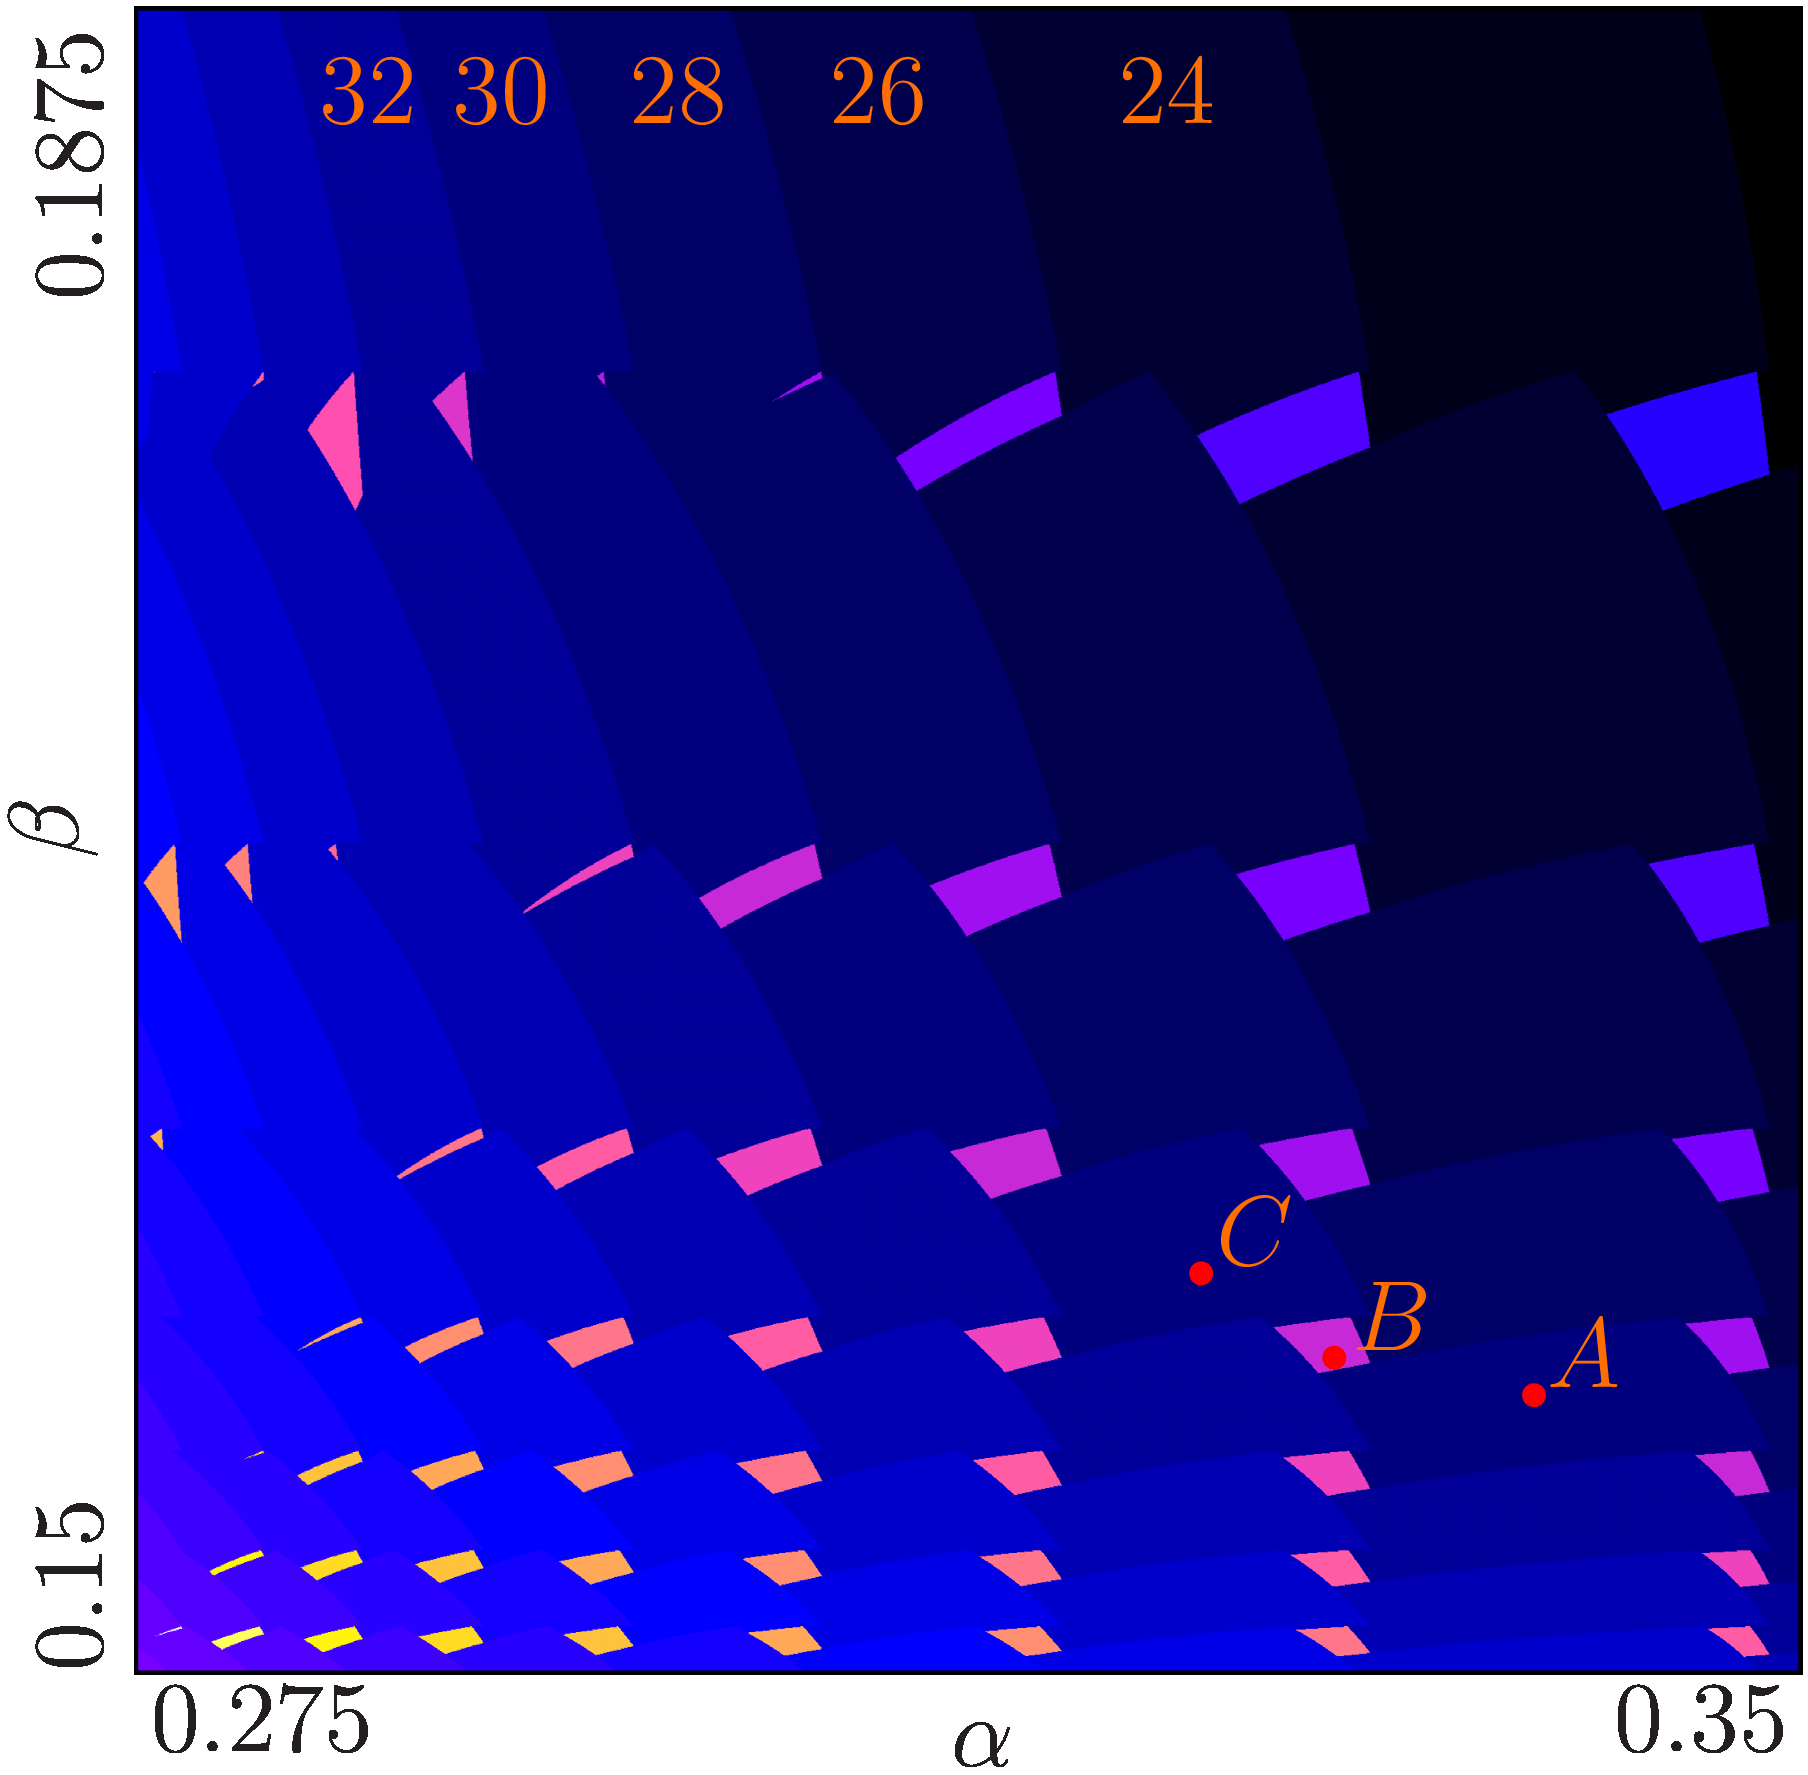
\includegraphics[width=.48\textwidth]{../Figures/5/5.11b/result.png}
		\label{fig:setup.quad.hyper.2.period.halved}
	}
	\caption[2D scan of the periods of the quadratic model with hyperparameters for different values of the fixed parameters]{
	2D scan of the periods of the piecewise quadratic model with hyperparameters $g_R\left(\frac{1}{4}\right), g_R\left(\frac{1}{2}\right),$ and $\left. \frac{d}{dx} g_R\left(x\right) \right|_{x = \frac{1}{2}}$.
	The parameters $a_L = 4, b_L = -\frac{1}{2}, g_R\left(\frac{1}{4}\right) = 0.525,$ and $\left. \frac{d}{dx} g_R\left(x\right) \right|_{x = \frac{1}{2}} = 1.2$ are fixed.
	The parameters $\alpha = g_R\left(\frac{1}{4}\right)$ and $\beta = c_L$ are varied in the ranges $[0.275, 0.35]$ and $[0.15, 0.1875]$, respectively.
	The points $A, B,$ and $C$ mark the parameter values used for the cobweb diagrams in \Cref{fig:setup.quad.hyper.2.cobwebs}.
	Also, the numbers at the top indicate the period of the parameter region chains.
	(a) shows the scan for the model as defined above, while (b) shows the scan for the halved model where we can see ``type B'' parameter regions as they have higher periods than the ``type A'' parameter regions of the same chain.
	}
	\label{fig:setup.quad.hyper.2.period}
\end{figure}

\begin{figure}
	\centering
	\subfloat[$A$]{
		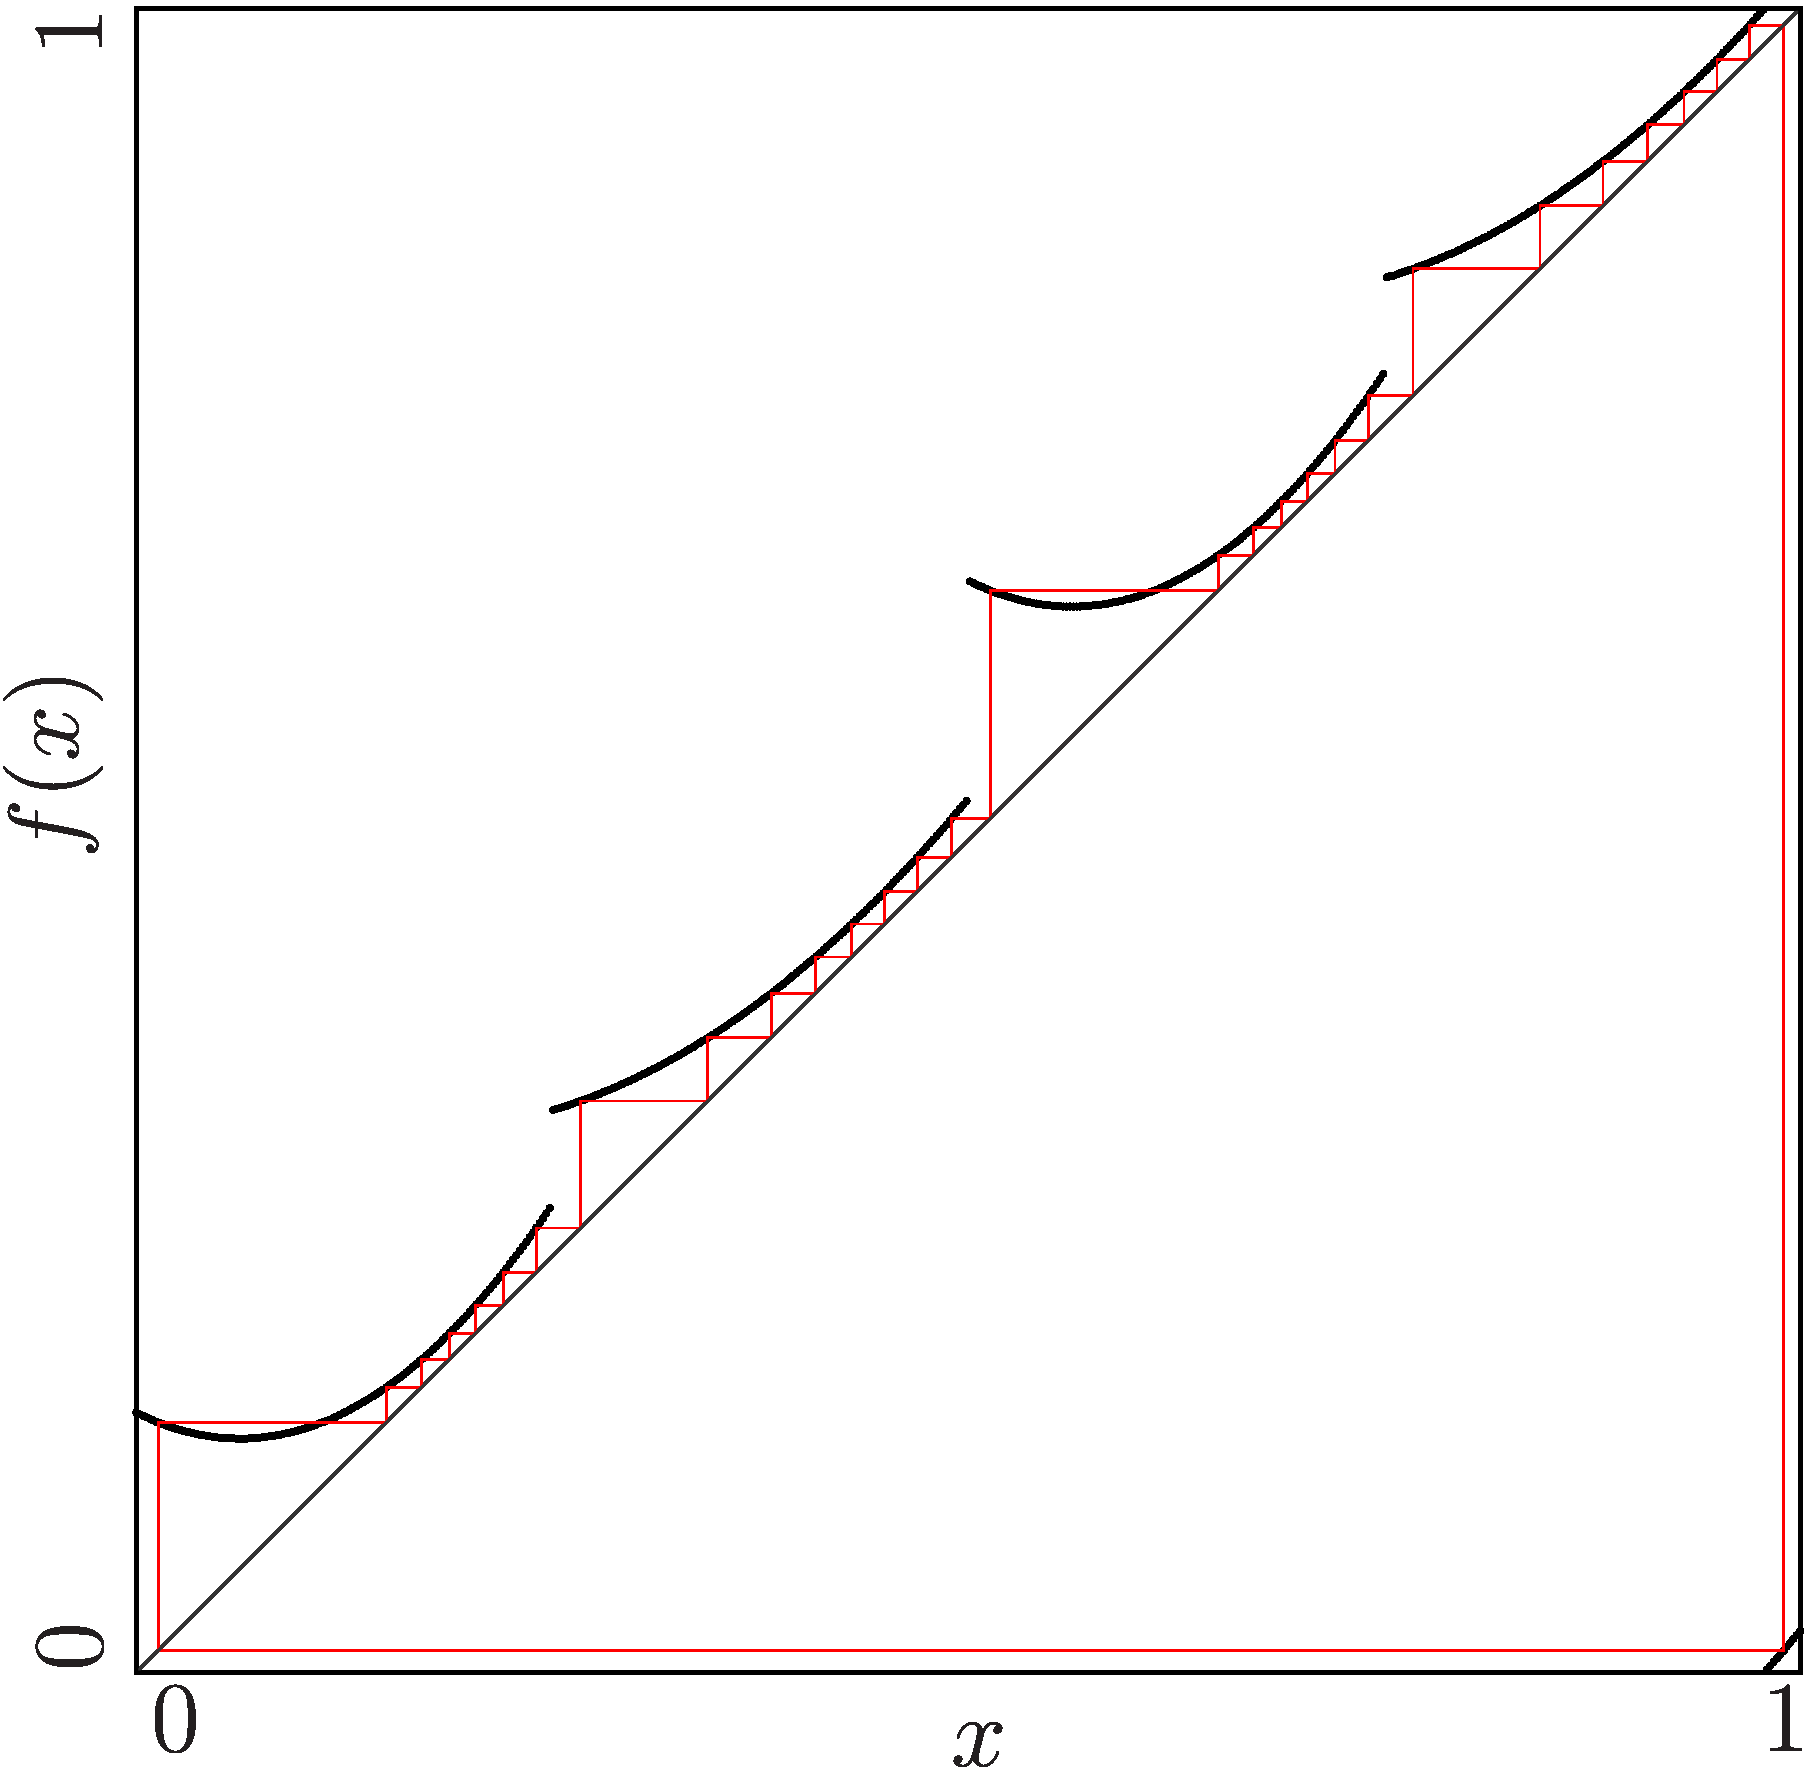
\includegraphics[width=.3 \textwidth]{../Figures/5/5.12a/result.png}
		\label{fig:setup.quad.hyper.2.cobweb.A}
	}
	\subfloat[$B$]{
		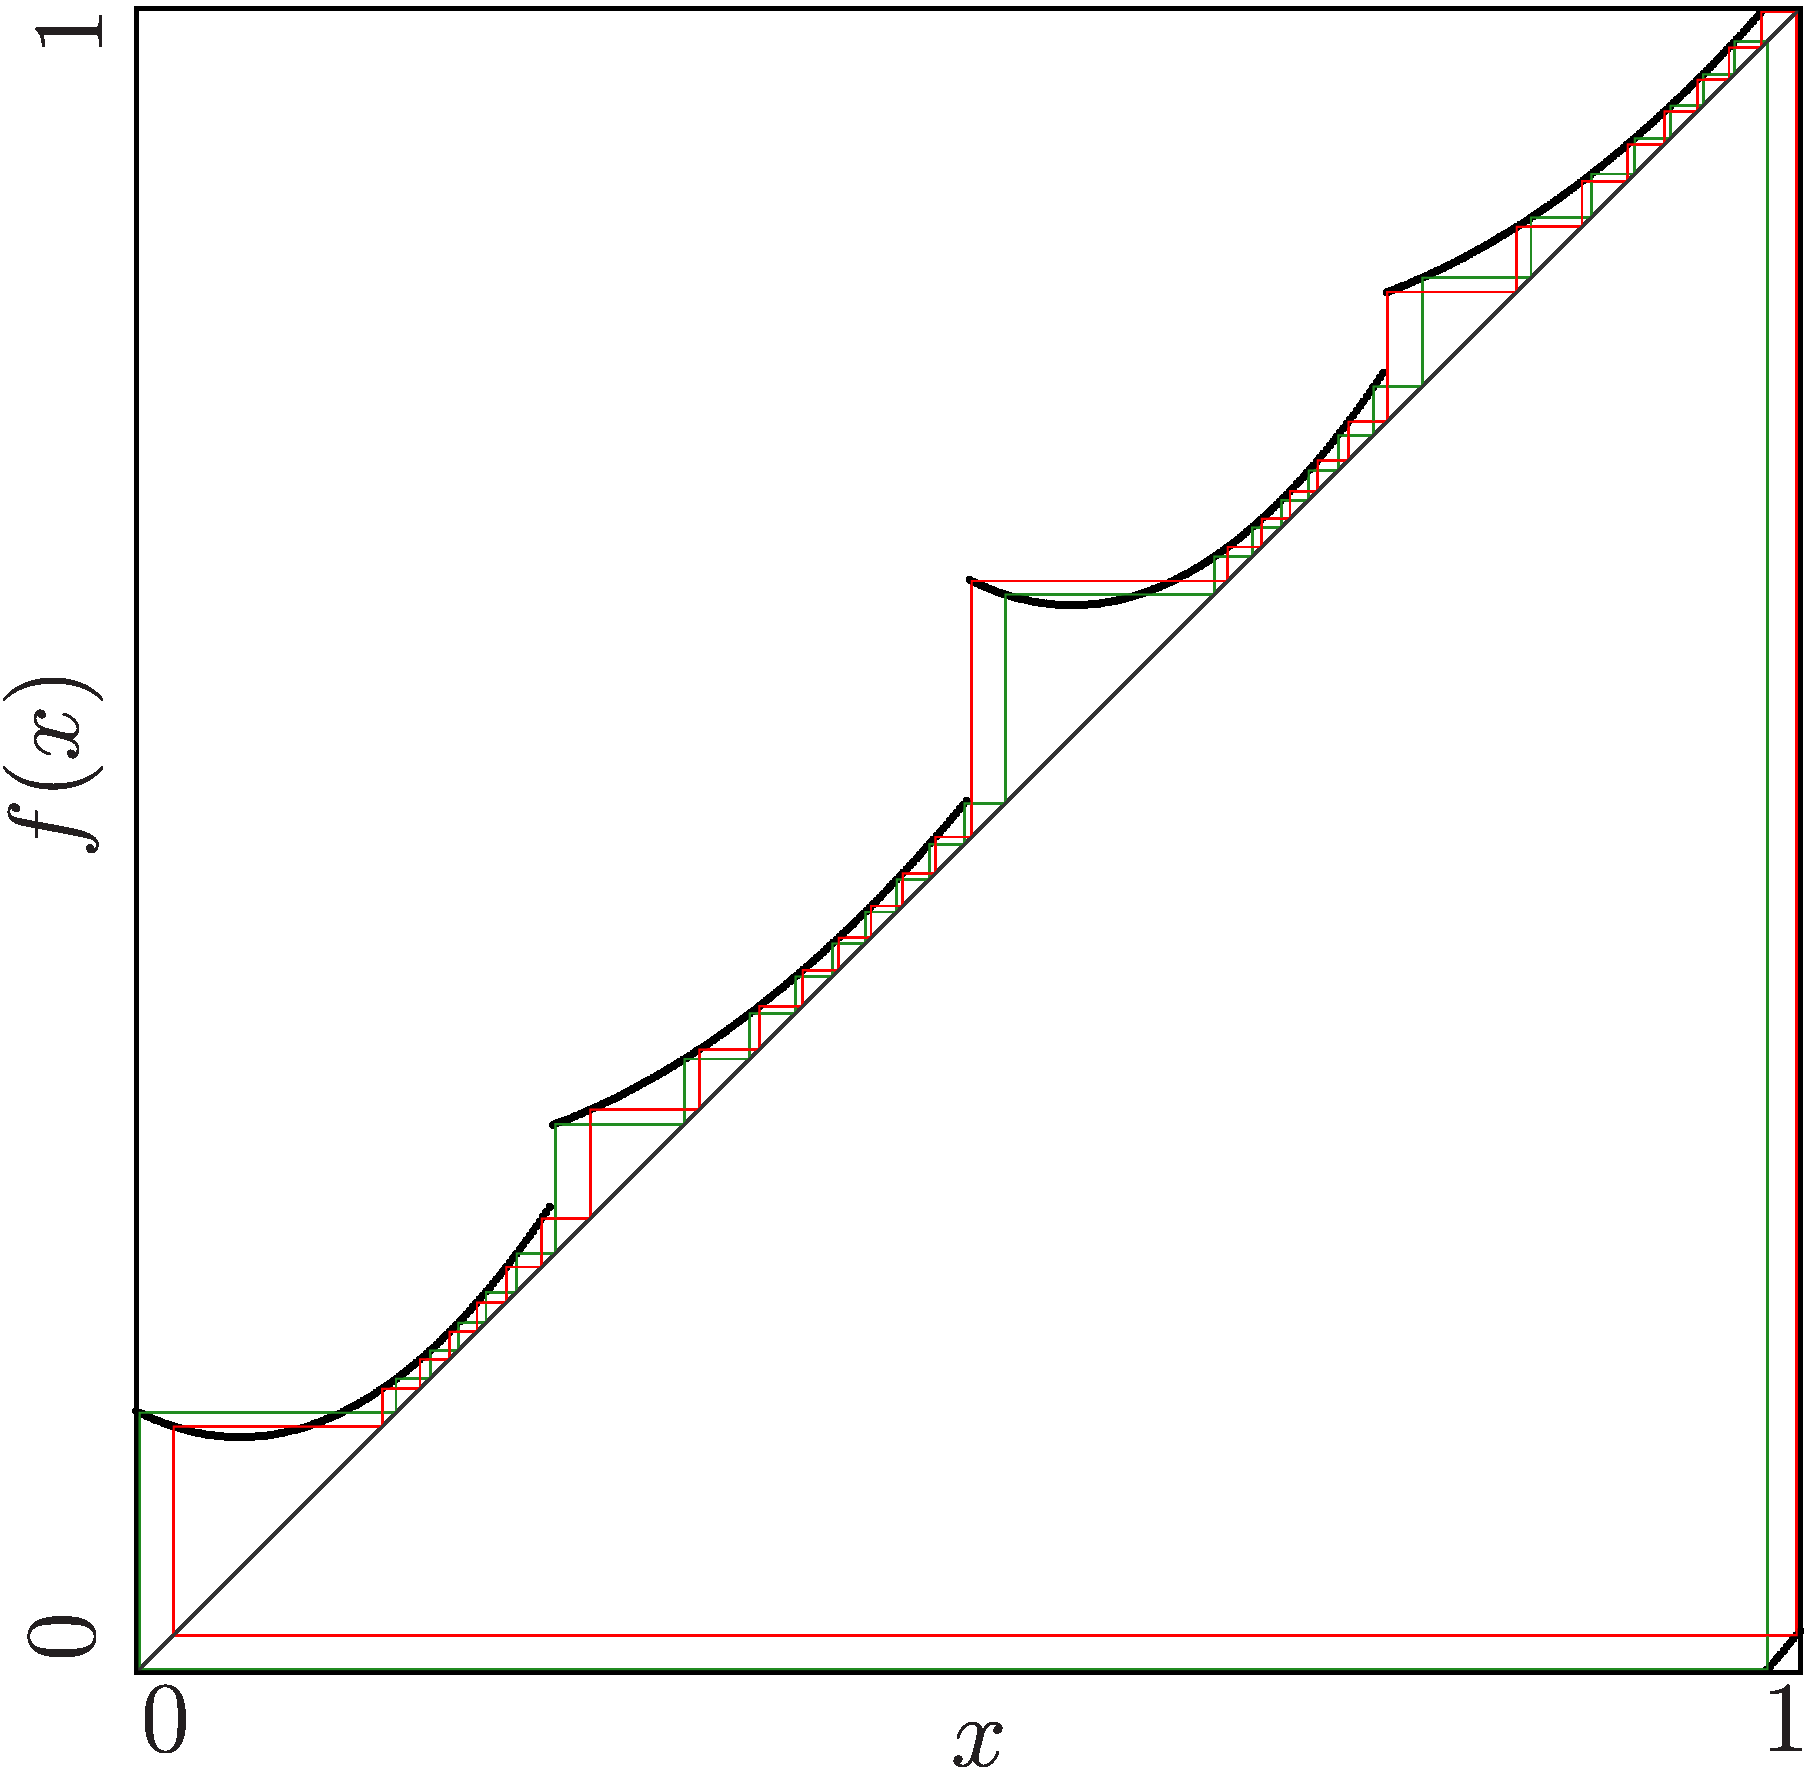
\includegraphics[width=.3 \textwidth]{../Figures/5/5.12b/result.png}
		\label{fig:setup.quad.hyper.2.cobweb.B}
	}
	\subfloat[$C$]{
		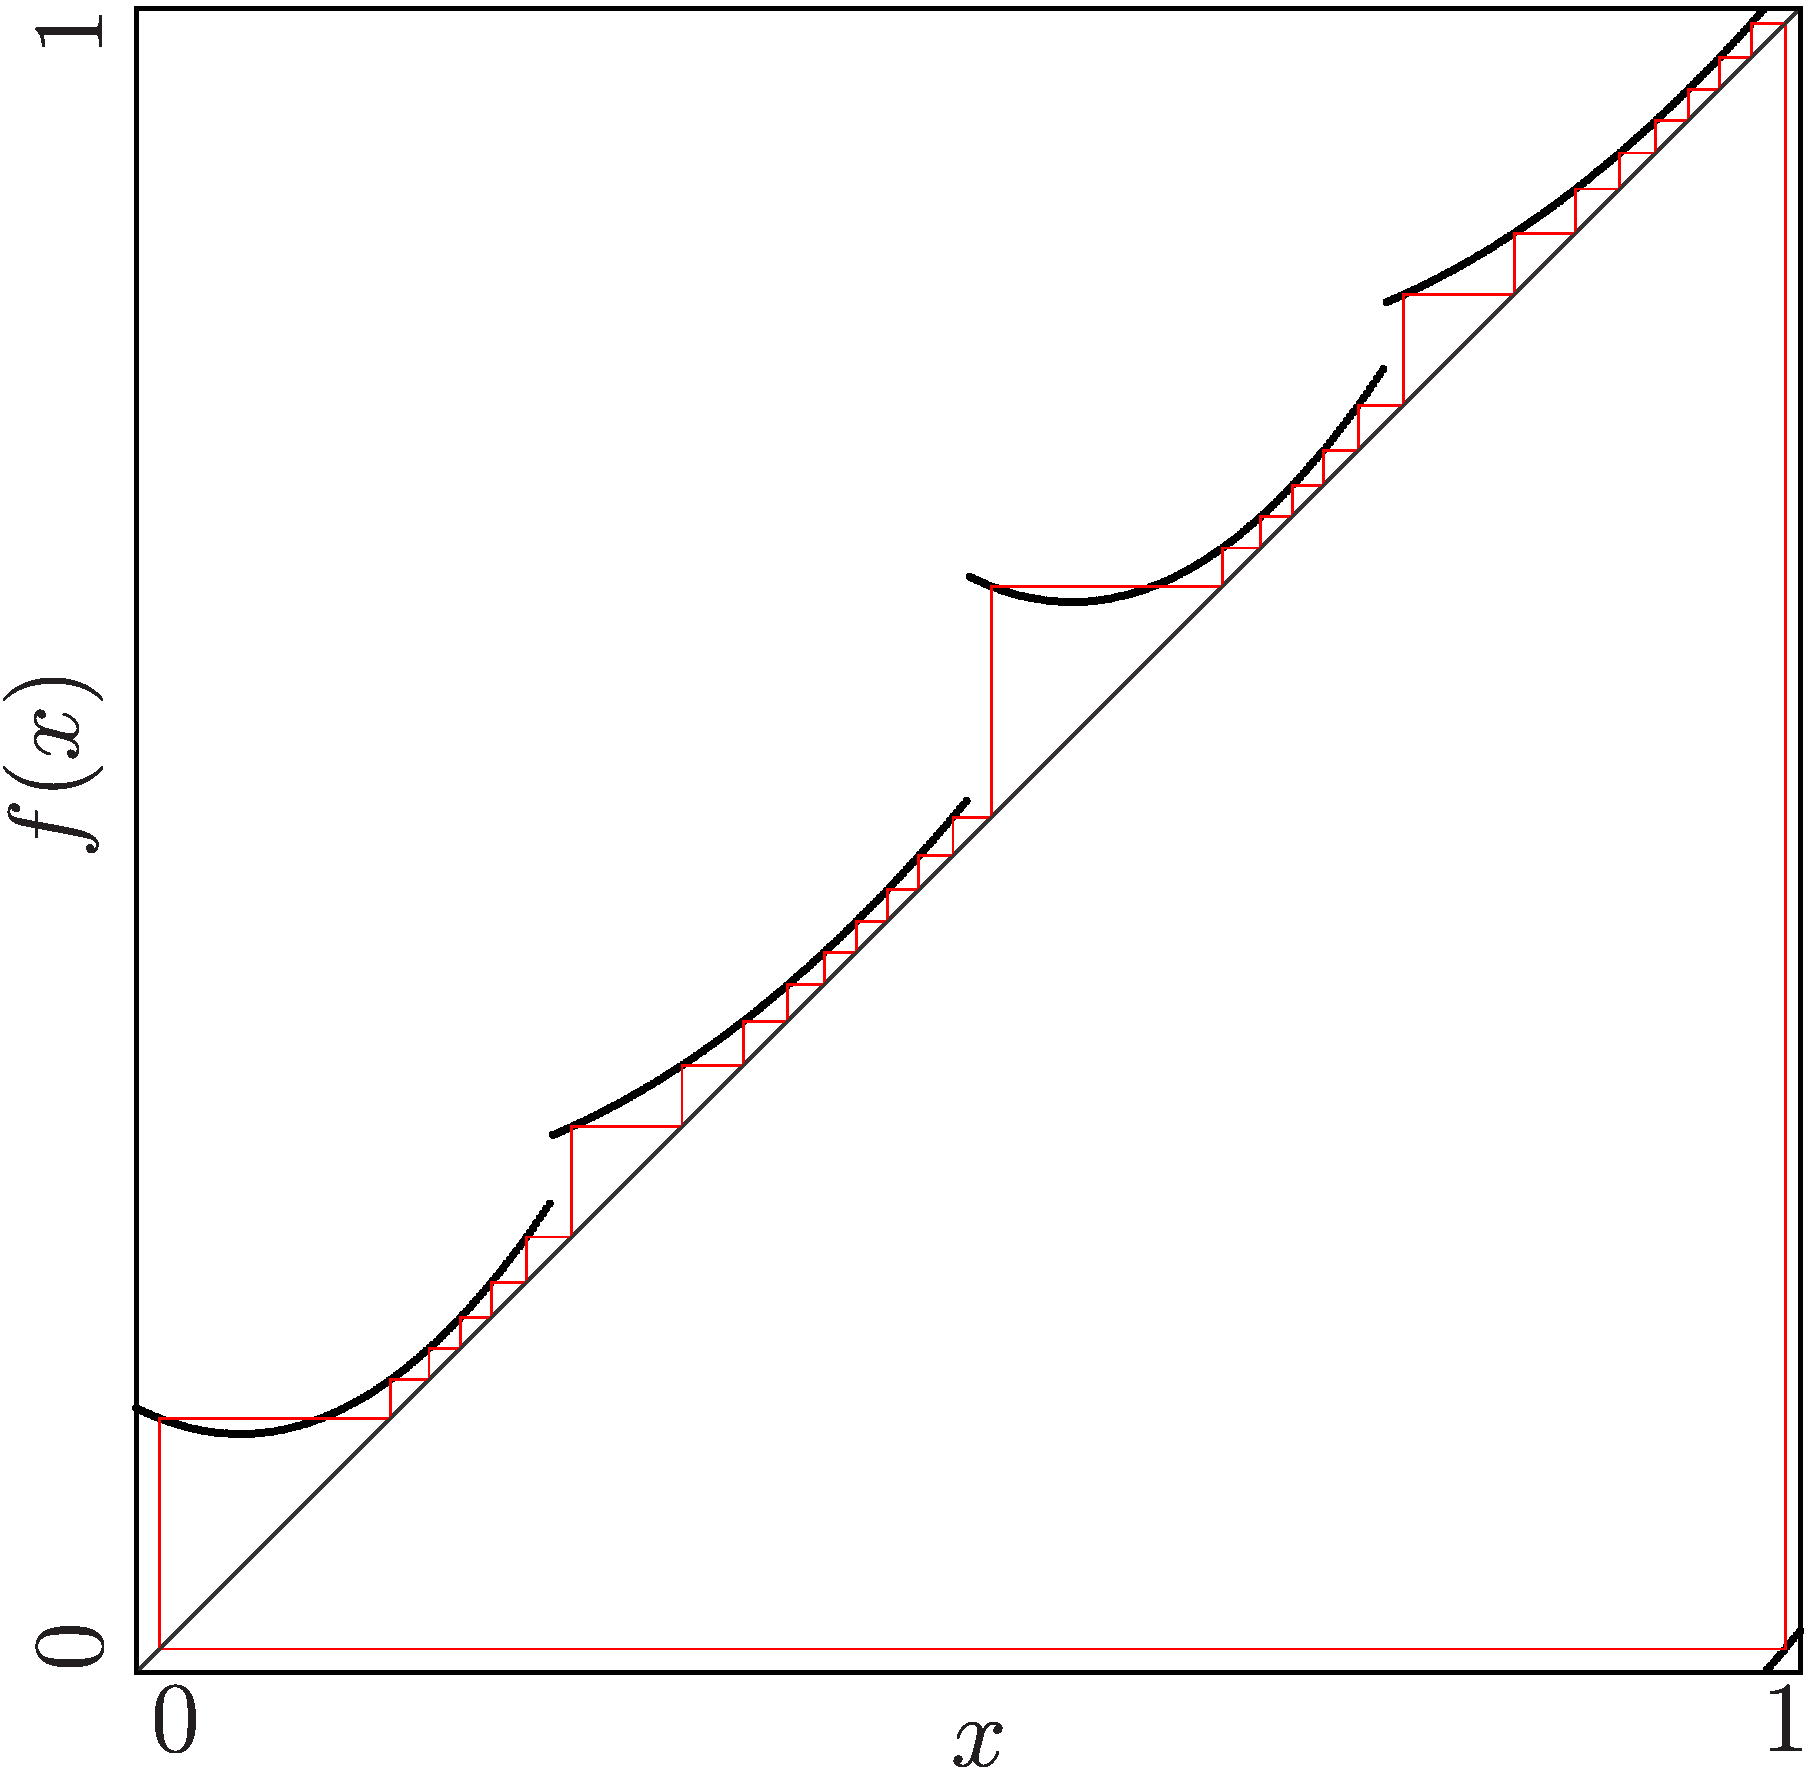
\includegraphics[width=.3 \textwidth]{../Figures/5/5.12c/result.png}
		\label{fig:setup.quad.hyper.2.cobweb.C}
	}
	\caption[Cobwebs of the piecewise quadratic model with hyperparameters for different values of the fixed parameters]{
	Cobweb diagrams at three parameter values of $\alpha = g_R\left(\frac{1}{4}\right)$ and $\beta = c_L$ in the piecewise quadratic model with hyperparameters.
	The other parameters are fixed as $a_L = 4, b_L = -\frac{1}{2}, g_R\left(\frac{1}{2}\right) = \frac{1}{2} + \frac{1}{40}$, and $\left. \frac{d}{dx} g_R(x) \right|_{x = \frac{1}{2}} = 1 + \frac{1}{5}$.
	The parameter values are marked in \Cref{fig:setup.quad.hyper.2.period}.
	(a) shows the cycle $\Cycle{\A^7\B^8\C^7\D^8}$ the at point $A$ \hl{where $\alpha = 0.338$ and $\beta = 0.15625$,}
	(b) shows the two coexisting cycles $\Cycle{\A^7\B^8\C^7\D^8}$ (green) and $\Cycle{\A^6\B^9\C^6\D^9}$ (red) at the point $B$ \hl{where $\alpha = 0.329$ and $\beta = 0.1571$,}
	and (c) shows the cycle $\Cycle{\A^6\B^9\C^6\D^9}$ at the point $C$ \hl{where $\alpha = 0.323$ and $\beta = 0.159$.}
	}
	\label{fig:setup.quad.hyper.2.cobwebs}
\end{figure}

\Cref{fig:setup.quad.hyper.2.cobwebs} contains the cobweb diagrams for \hl{the cycles at the parameter values that are marked with points $A, B,$ and $C$} in \Cref{fig:setup.quad.hyper.2.period}.
\hl{This chain of parameter regions is associated with the period $30$, therefore all the cycles shown here also have the period $30$}.
The symbolic sequence of the cycle at point $A$ is $\A^7\B^8\C^7\D^8$.
It is a symmetric cycle and therefore the parameter region is of ``type A''.
The symbolic sequence of the cycle at point $C$ is $\A^6\B^9\C^6\D^9$.
It is also a symmetric cycle and this parameter region is also of ``type A''.
\hl{
	The parameter region with point $C$ is the next ``type A'' parameter region after the parameter region with point $A$ in the chain.
	And just like in the original model, one point of each of the branches $f_\A$ and $f_\C$ moved to the next branch.
}

Between those two ``type A'' parameter regions there is a narrower \hl{``type B''} parameter region with the same period.
It is marked with the point $C$.
At this point, there are 2 coexisting cycles with the period 30.
Their symbolic sequences are $\A^7\B^8\C^6\D^9$ and $\A^6\B^9\C^7\D^8$, respectively.
This is exactly the same behavior that \hl{one can observe in the original model}.
\hl{
	Between two ``type A'' parameter regions with the cycles $\Cycle{\A^a\B^b\C^c\D^d}$ and $\Cycle{\A^c\B^d\C^c\D^d}$ there is a ``type B'' parameter region with the two coexisting cycles $\Cycle{\A^a\B^b\C^c\D^d}$ and $\Cycle{\A^c\B^d\C^c\D^d}$.
	Where $c = a - 1$ and $d = b + 1$.
}

\hl{
	Therefore, the bifurcation structure in this model fulfills all criteria, although it is mirrored.
	In the \gls{pi} structure in the original model, the periods increased from left to right, here they increase from right to left.
	Also, the chains start in the lower left corner and go towards to the upper right corner, here they start in the lower right corner and go towards the upper left corner.
	But the model can still be simplified.
	The branches $f_\B$ and $f_\D$ are only increasing and almost linear.
}
\hl{One can observe this in the cobweb diagrams in} \Cref{fig:setup.quad.hyper.2.cobwebs}.
